\documentclass[11pt]{article}

\title{Assignment 4: CS 763, Computer Vision}
\author{Ayush Baid (12D100002) \\
Niranjan Thakurdesai (12D100007) \\
Jainesh Doshi (12D070014)}
\date{Due 29th March before 11:55 pm}

\usepackage{amsmath}
\usepackage{graphicx}
\usepackage{amssymb}
\usepackage[margin=1in]{geometry}
\setlength\parindent{0pt}

\begin{document}
\maketitle

\section*{Question 1}

(See the Q1 folder for the complete report for Q1) \\
Recognition accuracies are as follows:
\begin{enumerate}
\item Dataset 1: 99.4\%
\item Dataset 2: 91.2\%
\item Dataset 3: 95.5\%
\item Dataset 4: 81.9\%
\item MNIST: 96.39\%
\end{enumerate}

\section*{Question 2}

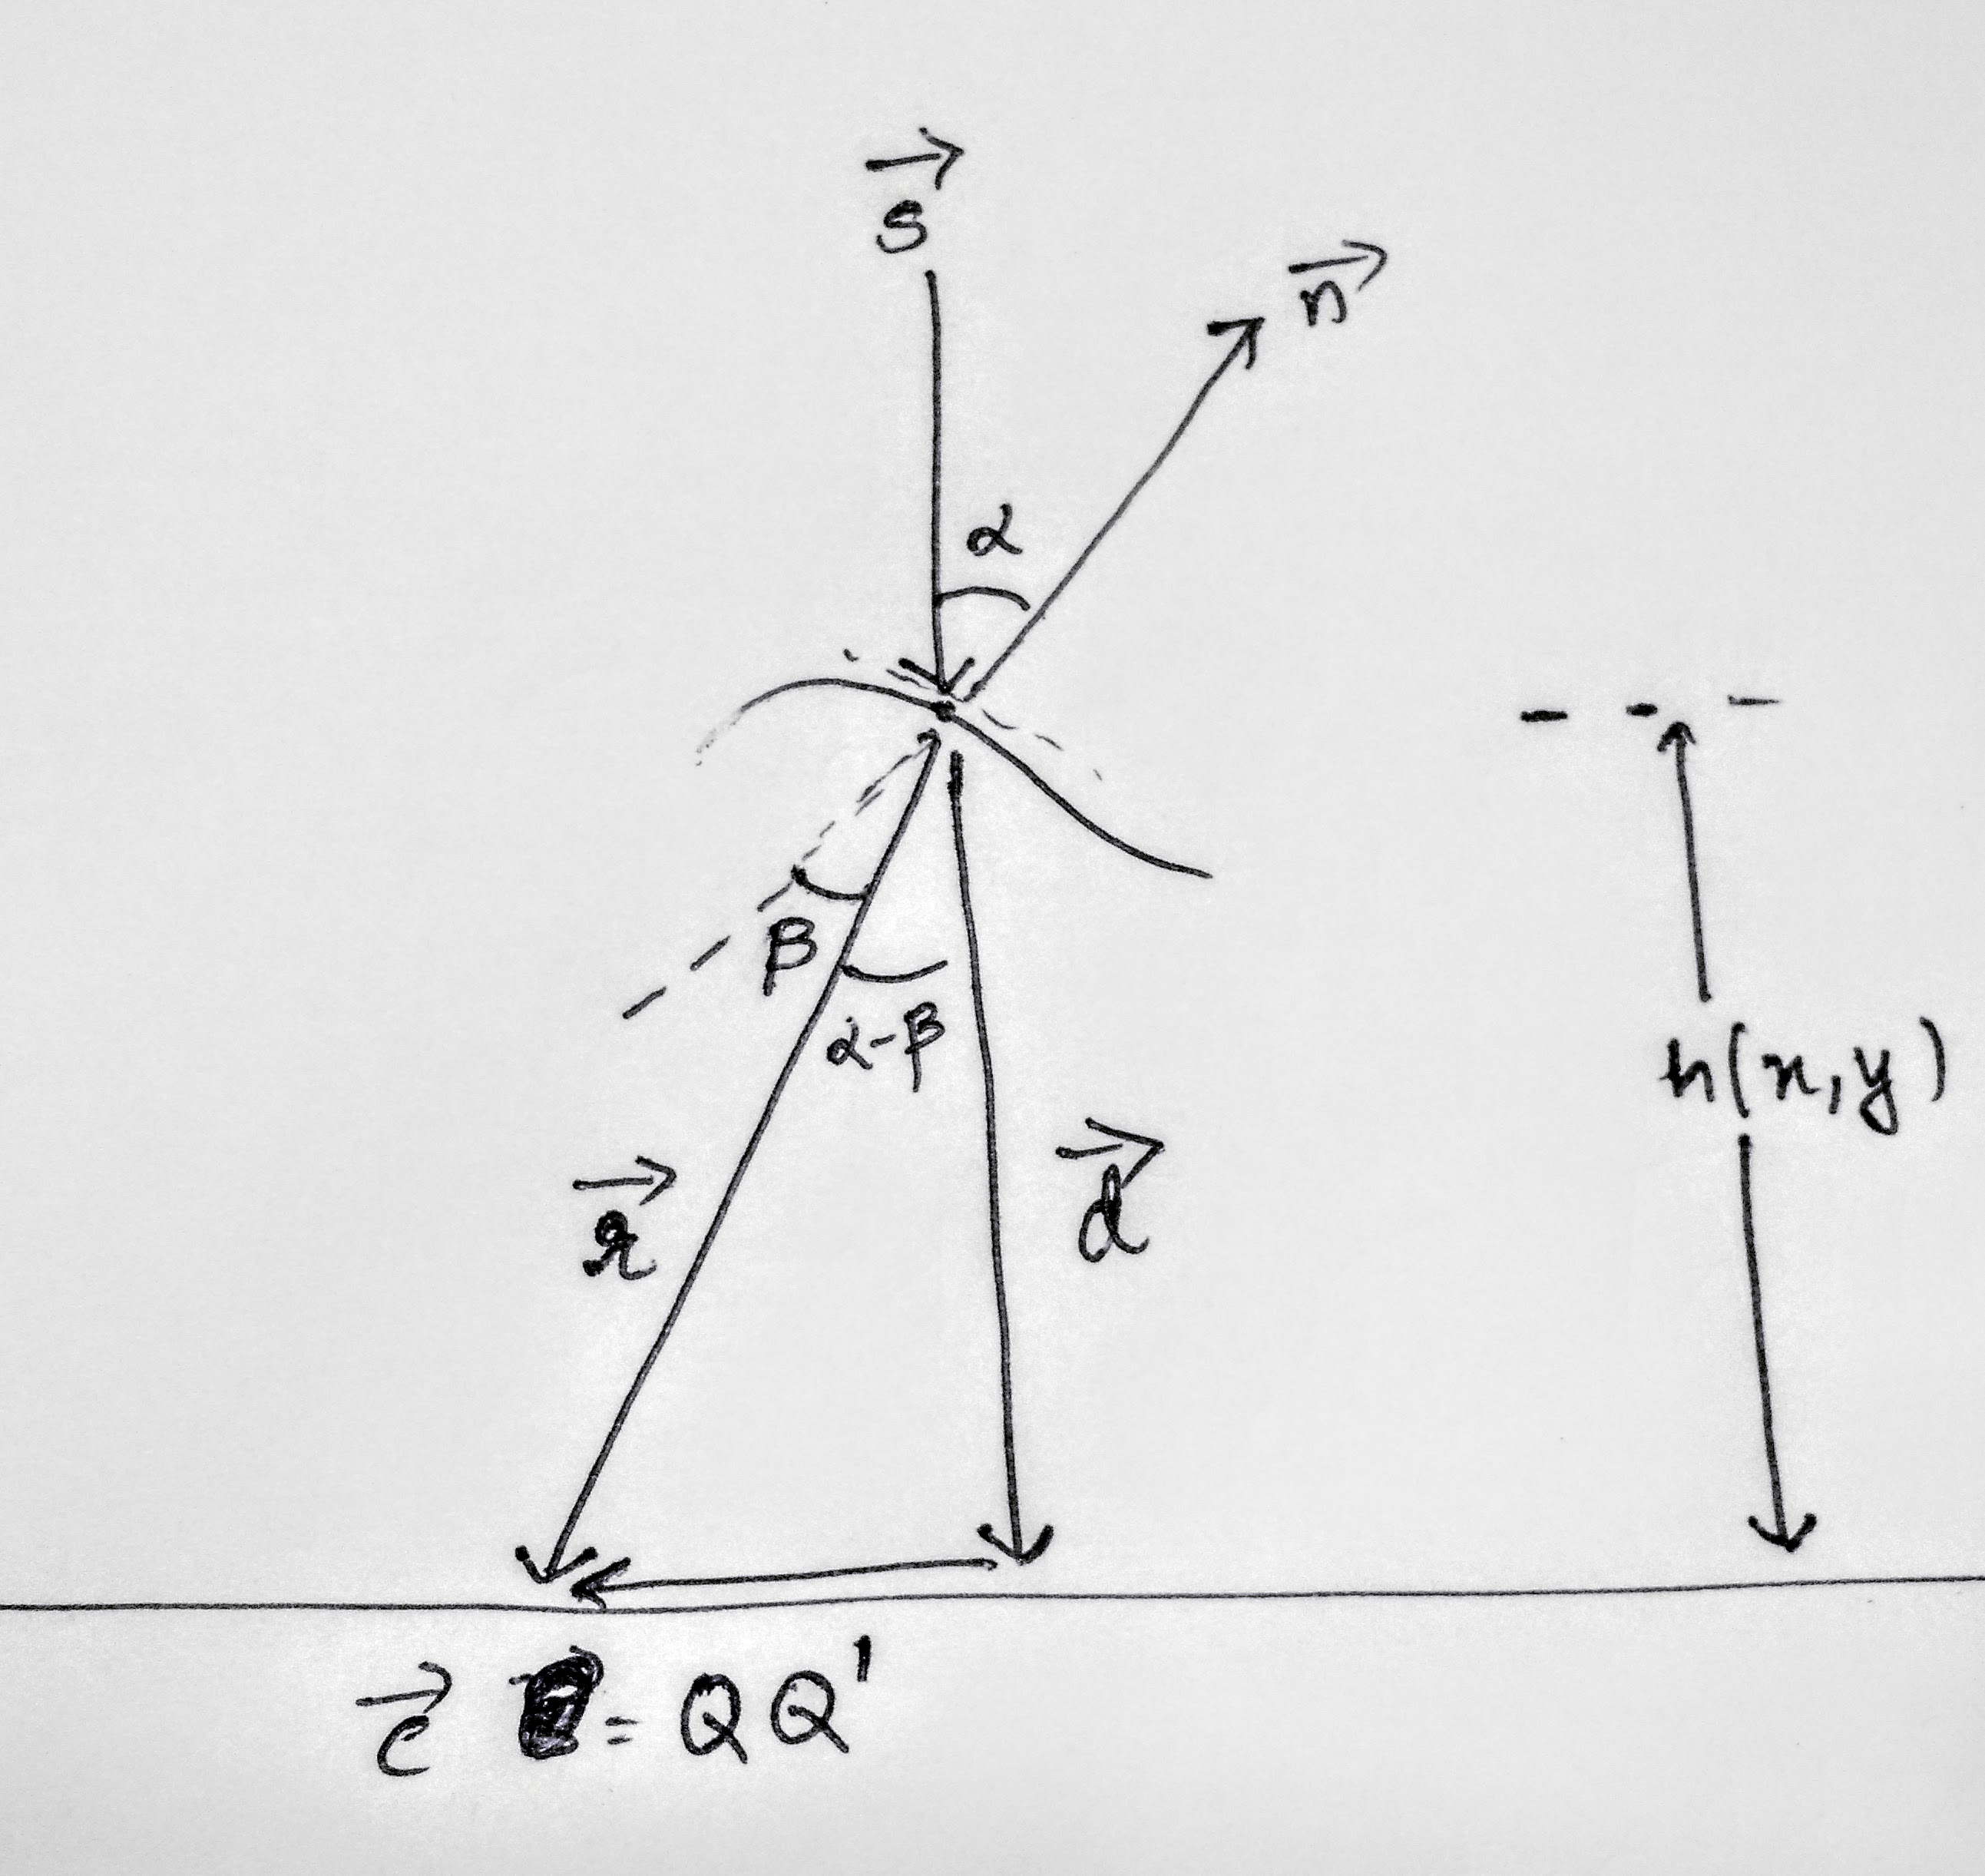
\includegraphics[scale=0.1]{diagram.jpg}

\subsection*{Part a}
Let the water surface have the equation $z = h(x,y)$. Thus, the normal to the surface is given by $\mathbf{n}(x,y) = \left( -\dfrac{\partial h}{\partial x},-\dfrac{\partial h}{\partial y},1 \right)$.\\

\subsection*{Part b}
As $\mathbf{s}$, $\mathbf{r}$ and $\mathbf{n}$ lie in the same plane, $(\mathbf{s}\times\mathbf{r})\cdot\mathbf{n}=0$. Now, $\mathbf{s} = (0,0,-1) \implies \mathbf{s}\times\mathbf{r} = (\mathbf{r}_y,-\mathbf{r}_x)$ and $\mathbf{n}(x,y) = \left( -\dfrac{\partial h}{\partial x},-\dfrac{\partial h}{\partial y},1 \right)$. Thus, we get $\frac{\mathbf{r}_y}{\mathbf{r}_x} = \left(\dfrac{\partial h}{\partial y}\right)/\left(\dfrac{\partial h}{\partial x}\right)$. Hence, $(\mathbf{r}_x,\mathbf{r}_y)$ is parallel to $(\dfrac{\partial h}{\partial x},\dfrac{\partial h}{\partial y})$.

\subsection*{Part c}
Note that $\mathbf{r}$, $\mathbf{c}$, and $\mathbf{d}$ are coplanar. Therefore, we can use basic trigonometry to estimate the magnitude of $\mathbf{c}$.

$|\mathbf{c}| = \tan(\alpha-\beta) * h(x,y)$. But h(x,y) will be close to $h_{0}$ and hence $|\mathbf{c}| \approxeq \tan(\alpha-\beta) * h_{0}$.

We can write two equations between $\mathbf{r}$ and $\mathbf{c}$ (QQ').\\
First equation is obtained by vector addition.
$$ \mathbf{d} + \mathbf{c} = \mathbf{r}$$.


Also, the angle between $\mathbf{r}$ and $\mathbf{c}$ is $90 - \alpha + \beta$

$$ \mathbf{r}.\mathbf{c} = ||\mathbf{r}||.||\mathbf{c}|| cos(90 - \alpha + \beta) $$

\subsection*{Part d}

$(h_{x},h_{y})$ is the projection of the surface normal on the XY plane. As the normal makes an angle $\alpha$ with the Z-axis, $||(h_{x},h_{y})|| = \sin\alpha$.\\

We have also established that $(\mathbf{r}_{x},\mathbf{r}_{y})$ is parallel to $(h_{x},h_{y})$.
\begin{gather*}
(\mathbf{r}_{x},\mathbf{r}_{y}) =  \frac{||(\mathbf{r}_{x},\mathbf{r}_{y})||}{||(h_{x},h_{y})||}(h_{x},h_{y}).
\end{gather*}

Since $\mathbf{c}$ is the projection of $\mathbf{r}$ on the XY plane,
\begin{gather*}
||\mathbf{c}|| = ||(r_{x},r_{y})|| \approx h_{0} sin(\alpha-\beta)
\end{gather*}


As $\alpha$, $\beta$ are small, and $h(x,y)$ is close to $h_{0}$, we can consider $||r|| \approx h_{0}$

\begin{gather*}
(\mathbf{r}_{x},\mathbf{r}_{y}) = \frac{h_{0} \sin(\alpha-\beta)}{\sin(\alpha)} (h_{x},h_{y})\\
(\mathbf{r}_{x},\mathbf{r}_{y}) = h_{0} \frac{\sin(\alpha)\cos(\beta) - \cos(\alpha)\sin(\beta)}{\sin(\alpha)} (h_{x},h_{y})\\
(\mathbf{r}_{x},\mathbf{r}_{y}) \approx (1-\frac{\sin\beta}{\sin\alpha}) (h_{x},h_{y})\\
(\mathbf{r}_{x},\mathbf{r}_{y}) \approx (1-\frac{1}{\kappa}) (h_{x},h_{y})\\
\end{gather*}

\subsection*{Part e}
Using Part d, $\mathbf{c} = \mathbf{r} - \mathbf{d}$. Also, as $\mathbf{c}$ is parallel to the XY plane, $\mathbf{c}_{z} = 0$. Hence, $\mathbf{c}_{x} = \mathbf{r}_{x}$ and $\mathbf{c}_{y} = \mathbf{r}_{y}$.

Also, we have the assumption that the time average depth of water at each point in $h_{0}$.\\

$
\implies \int_{t} h(x,y,t) dt = h_{0}   \text{ } \forall (x,y)
$\\
Taking derivatives w.r.t x and y,\\
$
\int_{t} \dfrac{\partial{h(x,y,t)}}{\partial{x}} dt = 0 \text{  and  } \int_{t} \dfrac{\partial{h(x,y,t)}}{\partial{y}} dt = 0   \text{ } \forall (x,y) 
$\\
$
\implies \int_{t} \mathbf{r}_{x} dt = 0 \text{ and } \int_{t} \mathbf{r}_{y} dt = 0 \text{ for all points. }
$\\
$\implies \int_{t} \mathbf{c} dt = 0 $ for all points.

Hence, for each point in the object, we can integrate its image in all frames and the take the average location as its true location. This will give us the actual location Q' for each point. Now, as we know $\mathbf{c} = QQ'$ and hence $\mathbf{r}_{x}$ and $\mathbf{r}_{x}$ at each point and at each frame, we get the partial derivatives $h_{x}$ and $h_{y}$.\\

We now have surface normals at each point, and can utilize shape from shading algorithm to recover the surface. The algorithm will give the surface but with an added constant, which can be different in each frame. We can utilize the property that the volume of water has to remain constant, hence the integration of $h(x,y)$ over the surface will remain constant at each frame. This correction will give us a consistent estimate across frames.
\end{document}